\documentclass[11pt]{exam}
\newcommand{\myname}{Xue Zhongkai} %Write your name in here
\newcommand{\myUCO}{122090636} %write your UCO in here
\newcommand{\myhwtype}{Homework}
\newcommand{\myhwnum}{4} %Homework set number
\newcommand{\myclass}{FIN2020}
\newcommand{\mylecture}{}
\newcommand{\mysection}{}

% Prefix for numedquestion's
\newcommand{\questiontype}{Question}

% Use this if your "written" questions are all under one section
% For example, if the homework handout has Section 5: Written Questions
% and all questions are 5.1, 5.2, 5.3, etc. set this to 5
% Use for 0 no prefix. Redefine as needed per-question.
\newcommand{\writtensection}{0}

\usepackage{amsmath, amsfonts, amsthm, amssymb}  % Some math symbols
\usepackage{enumerate}
\usepackage{enumitem}
\usepackage{graphicx}
\usepackage{hyperref}
\usepackage[all]{xy}
\usepackage{wrapfig}
\usepackage{fancyvrb}
\usepackage[T1]{fontenc}
\usepackage{listings}

\usepackage{centernot}
\usepackage{mathtools}
\DeclarePairedDelimiter{\ceil}{\lceil}{\rceil}
\DeclarePairedDelimiter{\floor}{\lfloor}{\rfloor}
\DeclarePairedDelimiter{\card}{\vert}{\vert}


\setlength{\parindent}{0pt}
\setlength{\parskip}{5pt plus 1pt}
\pagestyle{empty}

\def\indented#1{\list{}{}\item[]}
\let\indented=\endlist

\newcounter{questionCounter}
\newcounter{partCounter}[questionCounter]

\newenvironment{namedquestion}[1][\arabic{questionCounter}]{%
    \addtocounter{questionCounter}{1}%
    \setcounter{partCounter}{0}%
    \vspace{.2in}%
        \noindent{\bf #1}%
    \vspace{0.3em} \hrule \vspace{.1in}%
}{}

\newenvironment{numedquestion}[0]{%
	\stepcounter{questionCounter}%
    \vspace{.2in}%
        \ifx\writtensection\undefined
        \noindent{\bf \questiontype \; \arabic{questionCounter}. }%
        \else
          \if\writtensection0
          \noindent{\bf \questiontype \; \arabic{questionCounter}. }%
          \else
          \noindent{\bf \questiontype \; \writtensection.\arabic{questionCounter} }%
        \fi
    \vspace{0.3em} \hrule \vspace{.1in}%
}{}

\newenvironment{alphaparts}[0]{%
  \begin{enumerate}[label=\textbf{(\alph*)}]
}{\end{enumerate}}

\newenvironment{arabicparts}[0]{%
  \begin{enumerate}[label=\textbf{\arabic{questionCounter}.\arabic*})]
}{\end{enumerate}}

\newenvironment{questionpart}[0]{%
  \item
}{}

\newcommand{\answerbox}[1]{
\begin{framed}
\vspace{#1}
\end{framed}}

\pagestyle{head}

\headrule
\header{\textbf{\myclass\ \mylecture\mysection}}%
{\textbf{\myname\ (\myUCO)}}%
{\textbf{\myhwtype\ \myhwnum}}

\begin{document}
\thispagestyle{plain}
\begin{center}
  {\Large \myclass{} \myhwtype{} \myhwnum} \\
  \myname{} (\myUCO{}) \\
  \today
\end{center}


%Here you can enter answers to homework questions


% p1
\begin{numedquestion}
  If the economic is good, the final wealth is
  $$R_G = a(r_G+1) + (Y_0-a)(r_f+1)$$
  If it is bad, then 
  $$R_B = a(r_B+1) + (Y_0-a)(r_f+1)$$
  We have the expected utility to be
  $$E[u(\Tilde{R})] = \sum u_i p_i$$
  and specific utility function
  $$u(Y) = \ln(Y)$$
  Taking in the specific value, we get
  $$E[u(\Tilde{R})] = \frac{1}{2}\ln(110+0.2a)+\frac{1}{2}\ln(110-0.05a)$$
  Then the allocation problem is converted to the optimization problem as
  $$\max_{a} f(a) = \frac{1}{2}\ln(110+0.2a)+\frac{1}{2}\ln(110-0.05a)$$
  with the constraint
  $$0<a<100$$
  We have the F.O.C to be
  $$f'(a) = \frac{0.1}{110+0.2a}-\frac{0.025}{110-0.05a} = \frac{330-0.4a}{40(110+0.2a)(110-0.05a)} > 0$$
  which indicates $f(a)$ increases monotonically within the range.
  
  Thus we find the $a*$ to be $100$, so as to optimize $E[u(\Tilde{R})]$.
\end{numedquestion}

% p2
\begin{numedquestion}
  Assume the consumer decides to save $a \leq Y_0$ in stock, thus his consumption at $t = 0$ is
  $$c_0 = Y_0 - a$$
  In a good economy, his wealth at $t = 1$ is
  $$c_{1G} = a(1+r_G)$$
  In a bad one, his wealth at $t = 1$ is
  $$c_{1B} = a(1+r_B)$$
  Thus we have the expected utility to be
  $$f(a) = \ln(Y_0 - a) + \beta [\ln(a(1+r_G))\pi + \ln(a(1+r_B))(1-\pi)]$$
  With $f'(a) = 0$, we have
  $$a* = \frac{\beta Y_0}{\beta+1} < Y_0$$
  We find that the optimal saving has nothing to do with $\pi$, but this could not be generalized for any case.
\end{numedquestion}

\begin{numedquestion}
     \begin{alphaparts}
     \item We have the mean to be 
     $$\mu_z = \sum z_i p_i$$
     and the variance to be
     $$\sigma_z^2 = p_i \sum (z_i-\bar{z})^2$$
     With computation, we have
     $$\mu_{z1}=6.75 ,\sigma_{z1}^2=15.1875$$
     and 
     $$\mu_{z2}=5.36 ,\sigma_{z2}^2=4.2534$$
     It shows that
     $$\mu_{z1} > \mu_{z2}$$ 
     while
     $$\sigma_{z1}^2 > \sigma_{z2}^2$$
     No Mean-Variance Dominance.
     \item We draw the graph like:
     
     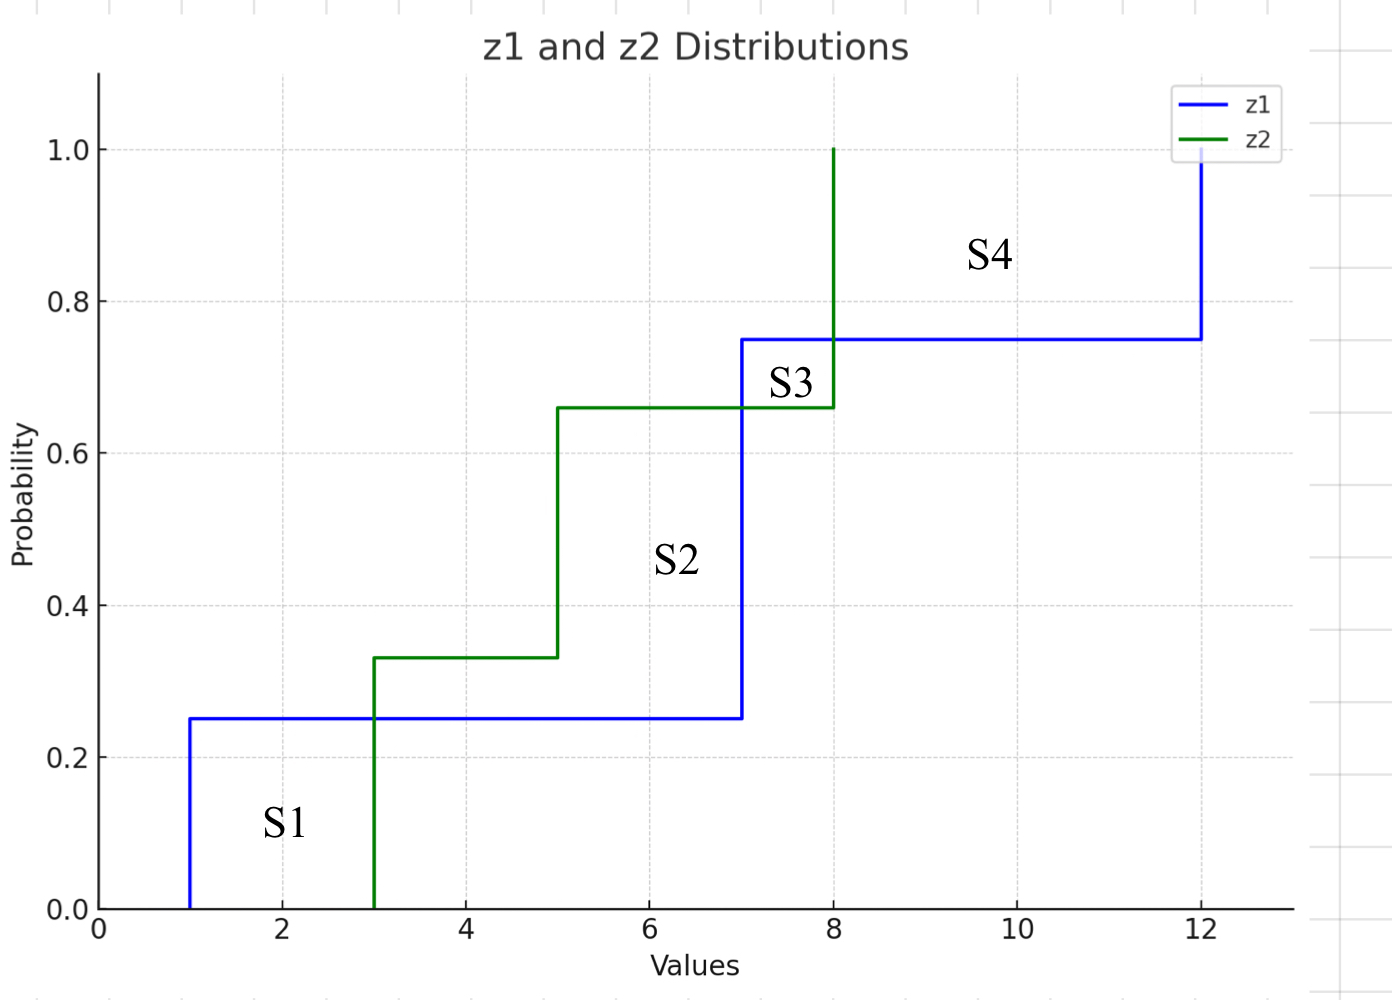
\includegraphics[width=0.5\textwidth]{1.jpeg}
     
     There is no $F_1 > F_2$ or $F_1 < F_2$ for every $z$.
     Thus there is no FOSD.
     \item The following $S_i$ represents $\int_{\Delta v} (F_1-F_2)dz$, as
     $$S_1 = 0.25 \times (3-1) = 0.5$$
     $$S_2 = (0.33-0.25) \times (5-3) + (0.66-0.25) \times (7-5)= -0.98$$
     $$S_3 = (0.75-0.66) \times (8-7) = 0.09$$
     $$S_4 = (1-0.75) \times (12-8) = -1$$
     Thus we have $G(z) = \int_{0}^{z} (F_1-F_2)dz$ to be
     $$G(1)=0$$
     $$G(3)=0.5$$
     $$G(7)=-0.48$$
     $$G(8)=-0.39$$
     $$G(12)=-1.39$$
     There is no $G(z) > 0$ or $G(z) \neq 0$ for every $z$, no SOSD.
     \end{alphaparts}
     
    \textbf{***This is the end of Homework 4.***}
\end{numedquestion}

\end{document}
